\documentclass[tikz,border=8pt,multi=tikzpicture]{standalone}
\usepackage{amsmath}
\usepackage{xcolor}
\usetikzlibrary{arrows.meta, calc}

\definecolor{mainblue}{HTML}{001158}
\definecolor{accent}{HTML}{8592bc}
\definecolor{lightaccent}{HTML}{e7e9f2}

\tikzset{
  force/.style={-{Stealth[length=3mm]}, line width=1.2pt, color=mainblue},
  dim/.style={-{Stealth[length=2mm]}, line width=0.7pt, color=accent},
  moment/.style={-{Stealth[length=2.5mm]}, line width=1.2pt, color=mainblue},
  member/.style={line width=1.4pt, color=mainblue},
  memberT/.style={line width=1.4pt, color=mainblue},
  memberC/.style={line width=1.4pt, color=accent},
  every node/.append style={font=\sffamily}
}

\newcommand{\festlager}[1]{
  \begin{scope}[shift={#1}]
    \draw[line width=1pt] (0,0) -- (-0.3,-0.5) -- (0.3,-0.5) -- cycle;
    \draw[line width=1pt] (-0.42,-0.5) -- (0.42,-0.5);
    \foreach \x in {-0.42,-0.24,...,0.42} {\draw[line width=0.4pt] (\x,-0.5) -- (\x-0.13,-0.68);}
  \end{scope}
}
\newcommand{\loslager}[1]{
  \begin{scope}[shift={#1}]
    \draw[line width=1pt] (0,0) -- (-0.3,-0.5) -- (0.3,-0.5) -- cycle;
    \foreach \x in {-0.18,0,0.18} {\draw[fill=white, line width=0.7pt] (\x,-0.6) circle (0.1);}
    \draw[line width=1pt] (-0.42,-0.72) -- (0.42,-0.72);
    \foreach \x in {-0.42,-0.24,...,0.42} {\draw[line width=0.4pt] (\x,-0.72) -- (\x-0.13,-0.9);}
  \end{scope}
}
\newcommand{\joint}[1]{\fill[mainblue] #1 circle (2.5pt);}

\begin{document}

% ================= Concept sketch: truss idealization =================
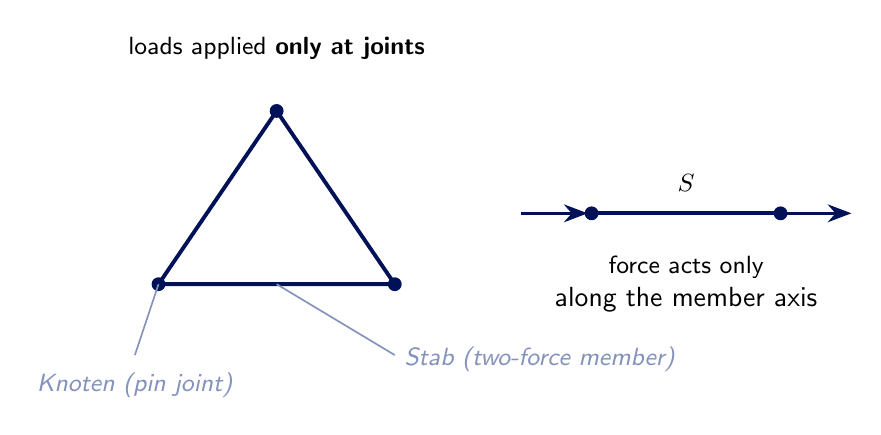
\begin{tikzpicture}
\coordinate (A) at (0,0); \coordinate (B) at (3,0); \coordinate (C) at (1.5,2.2);
\draw[member] (A) -- (B) -- (C) -- (A);
\joint{(A)} \joint{(B)} \joint{(C)}
\draw[accent, line width=0.6pt] (1.5,0) -- (3.0,-0.9);
\node[accent, right] at (3.0,-0.95) {\small \emph{Stab (two-force member)}};
\draw[accent, line width=0.6pt] (0,0) -- (-0.3,-0.9);
\node[accent, below] at (-0.3,-1.0) {\small \emph{Knoten (pin joint)}};
\node[align=center] at (1.5,3.0) {\small loads applied \textbf{only at joints}};
% inset: isolated two-force member
\begin{scope}[shift={(5.5,0.9)}]
\draw[member] (0,0) -- (2.4,0);
\joint{(0,0)} \joint{(2.4,0)}
\draw[force] (-0.9,0) -- (-0.05,0);
\draw[force] (2.45,0) -- (3.3,0);
\node[above] at (1.2,0.15) {\small $S$};
\node[align=center] at (1.2,-0.9) {\small force acts only \\ along the member axis};
\end{scope}
\end{tikzpicture}

% ================= Zero-force member rules =================
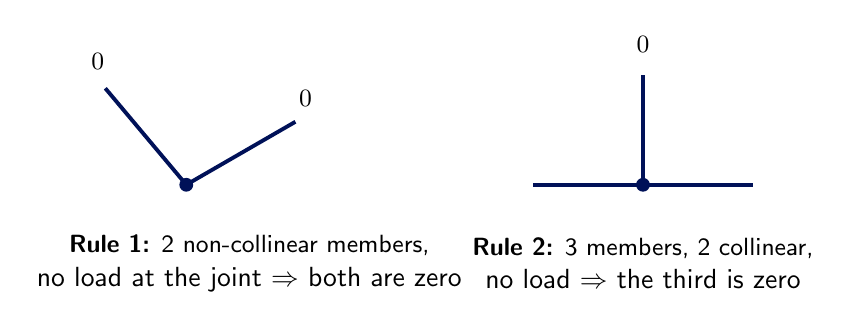
\begin{tikzpicture}
% rule (a): 2 non-collinear members, no load
\begin{scope}
\coordinate (O) at (0,0);
\draw[member] (O) -- ++(130:1.6);
\draw[member] (O) -- ++(30:1.6);
\joint{(O)}
\node[above] at (130:1.75) {\small $0$};
\node[above] at (30:1.75) {\small $0$};
\node[align=center] at (0.8,-1.0) {\small \textbf{Rule 1:} 2 non-collinear members,\\ no load at the joint $\Rightarrow$ both are zero};
\end{scope}
% rule (b): 3 members, 2 collinear, no load
\begin{scope}[shift={(5.8,0)}]
\coordinate (O) at (0,0);
\draw[member] (O) -- ++(180:1.4);
\draw[member] (O) -- ++(0:1.4);
\draw[member] (O) -- ++(90:1.4);
\joint{(O)}
\node[above] at (90:1.55) {\small $0$};
\node[align=center] at (0,-1.0) {\small \textbf{Rule 2:} 3 members, 2 collinear,\\ no load $\Rightarrow$ the third is zero};
\end{scope}
\end{tikzpicture}

% ================= Ex 5.1 problem: simple triangular truss =================
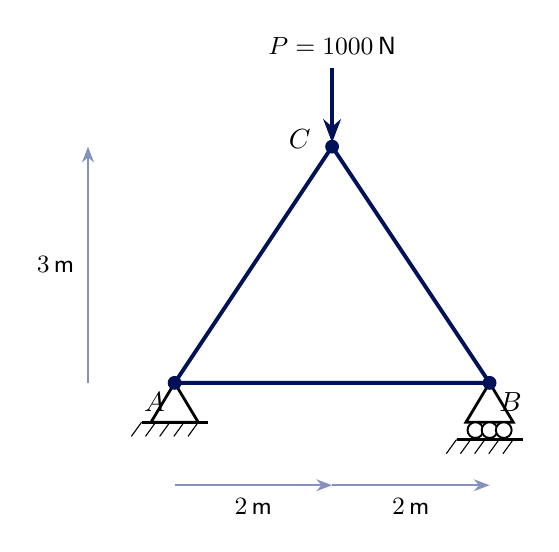
\begin{tikzpicture}
\coordinate (A) at (0,0); \coordinate (B) at (4,0); \coordinate (C) at (2,3);
\festlager{(A)}
\loslager{(B)}
\draw[member] (A) -- (B) -- (C) -- (A);
\joint{(A)} \joint{(B)} \joint{(C)}
\node[below left] at (A) {$A$};
\node[below right] at (B) {$B$};
\node[left] at ($(C)+(-0.15,0.1)$) {$C$};
\draw[force] (2,4.0) -- (2,3.05);
\node[above] at (2,4.05) {\small $P=1000\,\text{N}$};
\draw[dim] (0,-1.3) -- (2,-1.3);
\node[below] at (1,-1.35) {\small $2\,\text{m}$};
\draw[dim] (2,-1.3) -- (4,-1.3);
\node[below] at (3,-1.35) {\small $2\,\text{m}$};
\draw[dim] (-1.1,0) -- (-1.1,3);
\node[left] at (-1.15,1.5) {\small $3\,\text{m}$};
\end{tikzpicture}

% ================= Ex 5.1 joint B free body =================
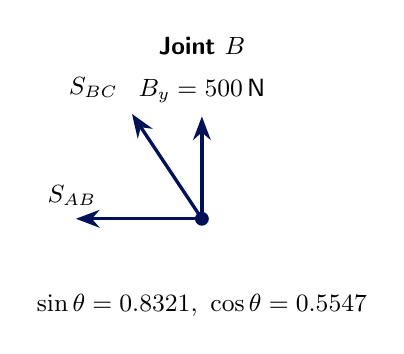
\begin{tikzpicture}
\node[align=center] at (0,2.2) {\small \textbf{Joint $B$}};
\joint{(0,0)}
\draw[force] (0,0.05) -- (0,1.3);
\node[above] at (0,1.35) {\small $B_y=500\,\text{N}$};
\draw[force] (0,0) -- ++(180:1.6);
\node[above] at (-1.65,0.05) {\small $S_{AB}$};
\draw[force] (0,0) -- ++(123.7:1.6);
\node[above left] at (123.7:1.7) {\small $S_{BC}$};
\node at (0,-1.1) {\small $\sin\theta=0.8321,\ \cos\theta=0.5547$};
\end{tikzpicture}

% ================= Ex 5.1 joint A free body =================
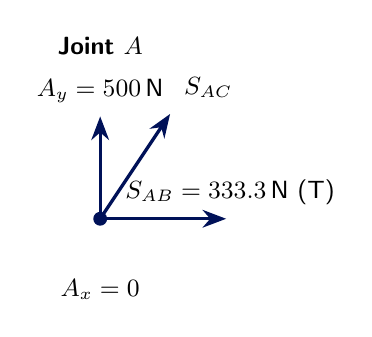
\begin{tikzpicture}
\node[align=center] at (0,2.2) {\small \textbf{Joint $A$}};
\joint{(0,0)}
\draw[force] (0,0.05) -- (0,1.3);
\node[above] at (0,1.35) {\small $A_y=500\,\text{N}$};
\draw[force] (0,0) -- ++(0:1.6);
\node[above] at (1.65,0.05) {\small $S_{AB}=333.3\,\text{N (T)}$};
\draw[force] (0,0) -- ++(56.3:1.6);
\node[above right] at (56.3:1.7) {\small $S_{AC}$};
\node at (0,-0.9) {\small $A_x=0$};
\end{tikzpicture}

% ================= Ex 5.2 problem: two-triangle truss, off-centre apex load =================
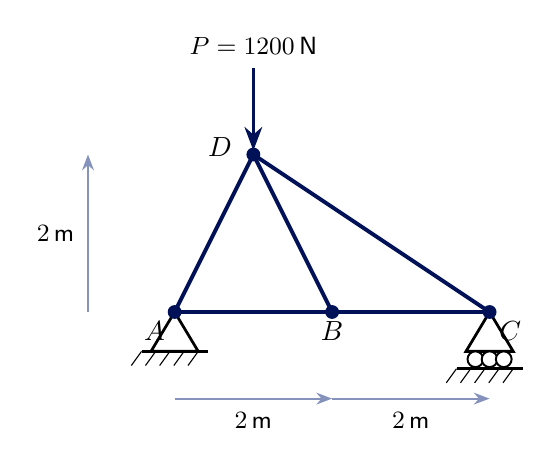
\begin{tikzpicture}
\coordinate (A) at (0,0); \coordinate (B) at (2,0); \coordinate (C) at (4,0); \coordinate (D) at (1,2);
\festlager{(A)}
\loslager{(C)}
\draw[member] (A) -- (B) -- (C);
\draw[member] (A) -- (D) -- (B);
\draw[member] (D) -- (C);
\joint{(A)} \joint{(B)} \joint{(C)} \joint{(D)}
\node[below left] at (A) {$A$};
\node[below] at (B) {$B$};
\node[below right] at (C) {$C$};
\node[left] at ($(D)+(-0.15,0.1)$) {$D$};
\draw[force] (1,3.1) -- (1,2.05);
\node[above] at (1,3.15) {\small $P=1200\,\text{N}$};
\draw[dim] (0,-1.1) -- (2,-1.1);
\node[below] at (1,-1.15) {\small $2\,\text{m}$};
\draw[dim] (2,-1.1) -- (4,-1.1);
\node[below] at (3,-1.15) {\small $2\,\text{m}$};
\draw[dim] (-1.1,0) -- (-1.1,2);
\node[left] at (-1.15,1) {\small $2\,\text{m}$};
\end{tikzpicture}

% ================= Ex 5.2 solved: forces annotated on members =================
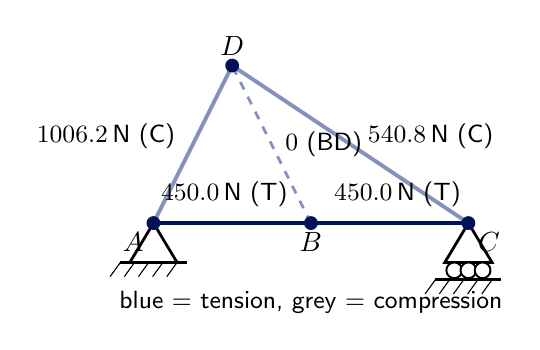
\begin{tikzpicture}
\coordinate (A) at (0,0); \coordinate (B) at (2,0); \coordinate (C) at (4,0); \coordinate (D) at (1,2);
\festlager{(A)}
\loslager{(C)}
\draw[memberT] (A) -- (B);
\draw[memberT] (B) -- (C);
\draw[accent, dashed, line width=1pt] (B) -- (D);
\draw[memberC] (A) -- (D);
\draw[memberC] (D) -- (C);
\joint{(A)} \joint{(B)} \joint{(C)} \joint{(D)}
\node[below left] at (A) {$A$};
\node[below] at (B) {$B$};
\node[below right] at (C) {$C$};
\node[above] at (D) {$D$};
\node[above] at (0.9,0.08) {\small $450.0\,\text{N (T)}$};
\node[above] at (3.1,0.08) {\small $450.0\,\text{N (T)}$};
\node[left] at (0.4,1.1) {\small $1006.2\,\text{N (C)}$};
\node[right] at (2.6,1.1) {\small $540.8\,\text{N (C)}$};
\node[right] at (1.55,1.0) {\small $0$ (BD)};
\node at (2,-1.0) {\small blue = tension, grey = compression};
\end{tikzpicture}

% ================= Ex 5.3 problem: triangular truss, horizontal joint load =================
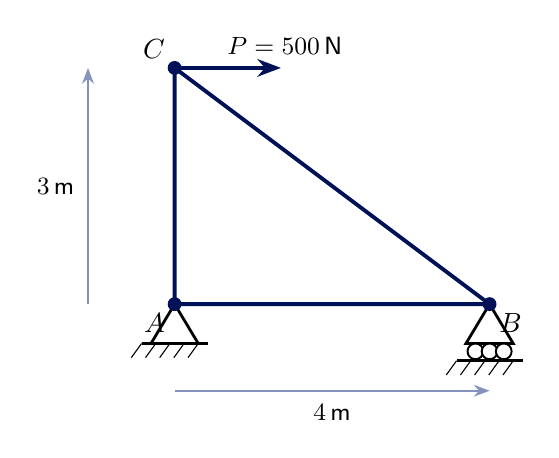
\begin{tikzpicture}
\coordinate (A) at (0,0); \coordinate (B) at (4,0); \coordinate (C) at (0,3);
\festlager{(A)}
\loslager{(B)}
\draw[member] (A) -- (B) -- (C) -- (A);
\joint{(A)} \joint{(B)} \joint{(C)}
\node[below left] at (A) {$A$};
\node[below right] at (B) {$B$};
\node[above left] at (C) {$C$};
\draw[force] (0.05,3) -- (1.35,3);
\node[above] at (1.4,3.05) {\small $P=500\,\text{N}$};
\draw[dim] (0,-1.1) -- (4,-1.1);
\node[below] at (2,-1.15) {\small $4\,\text{m}$};
\draw[dim] (-1.1,0) -- (-1.1,3);
\node[left] at (-1.15,1.5) {\small $3\,\text{m}$};
\end{tikzpicture}

% ================= Ex 5.3 solved: forces annotated on members =================
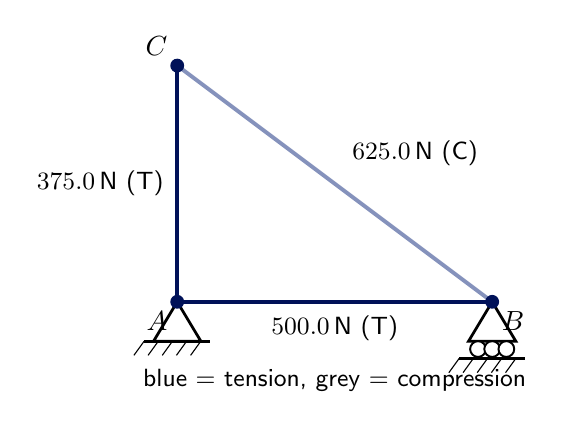
\begin{tikzpicture}
\coordinate (A) at (0,0); \coordinate (B) at (4,0); \coordinate (C) at (0,3);
\festlager{(A)}
\loslager{(B)}
\draw[memberT] (A) -- (B);
\draw[memberT] (A) -- (C);
\draw[memberC] (B) -- (C);
\joint{(A)} \joint{(B)} \joint{(C)}
\node[below left] at (A) {$A$};
\node[below right] at (B) {$B$};
\node[above left] at (C) {$C$};
\node[below] at (2,-0.05) {\small $500.0\,\text{N (T)}$};
\node[left] at (-0.05,1.5) {\small $375.0\,\text{N (T)}$};
\node[above right] at (2.1,1.6) {\small $625.0\,\text{N (C)}$};
\node at (2,-1.0) {\small blue = tension, grey = compression};
\end{tikzpicture}

\end{document}
